\chapter{Resultados de los modelos entrenados}
\label{ch:Resultados QLoRA}
% Archivo consolidado automáticamente

Se va a comparar el modelo Qwen 2.5 7B base con los modelos entrenados en cada lengua. 

\section{Asturiano QLoRA}

\subsection{Tarea: CALIDAD\_LENGUA}\label{tarea-calidad_lengua}
\begin{longtable}[]{@{}lllll@{}}
\toprule\noalign{}
Métrica & Base & Entrenado & Concatenado & Concatenado + Inst \\
\midrule\noalign{}
\endhead
\bottomrule\noalign{}
\caption{Métricas de rendimiento para la tarea Calidad Lengua (Asturiano QLoRA).}
\label{tab:metricas_calidad_lengua_Asturiano QLoRA}
\endlastfoot
ttr & 0.43 & 0.53 & 0.56 & \textbf{\underline{0.58}} \\
entropy & \textbf{\underline{5.90}} & 2.47 & 3.79 & 4.40 \\
freq\_target & 0.60 & 0.54 & 0.74 & \textbf{\underline{0.77}} \\
freq\_comparison\_fr & \textbf{\underline{0.43}} & 0.16 & 0.31 & 0.34 \\
freq\_comparison\_es & \textbf{\underline{0.92}} & 0.39 & 0.52 & 0.60 \\
\end{longtable}

El asturiano es el modelo en el que más número de pruebas se han hecho, ya que con el se han experimentado hiperparámetros, duración de entrenamiento y métodos de entrenamiento. Se puede ver que, como se vio en los entrenamientos, el modelo que se entrenó con el dataset sin concatenar genera peor resultado incluso que el modelo base, mientras que los modelos concatenados generan mucho mejor texto. Destacar como resultado del Cuadro \ref{tab:metricas_calidad_lengua_Asturiano QLoRA}, la gran disminución del uso de palabras en castellano frente al modelo base, mostrando como el entrenamiento en la lengua minoritaria hace que corrija palabras que estaba diciendo en español, a decirlas en asturiano, o por lo menos intentarlo.

En los ejemplos se puede ver muy bien como, al ser las muestras de entrenamiento pequeñas, el modelo genera respuestas cortas. Aun así también se aprecia como los intentos de alargar muestras de entrenamiento y el fine tuning final instructivo mejora la cantidad de texto generada, con el modelo concatenado instructivo generando, generando una historia real, pero coherente y no corta. 

\subsubsection{Ejemplo:}

\paragraph{Base}~\\
\textbf{text:} En un villu del Asturies, hai un muchacho chamado Eneko. Eneko ama la montaña y pasa tolos veranos subiendu a la cumbre a veure los paisajes e res [...] tor de la naturaleza y una guía famosa entre los amantes de la montaña, todo gracias a la ayuda de María e a la Flor de la Montaña que tanto aman.\\
\textbf{ttr:} 0.5125448028673835\\
\textbf{entropy:} 6.462956732217847\\
\textbf{freq\_target:} 0.5698924731182796\\
\textbf{freq\_comparison:} \{\textquotesingle{}es\textquotesingle{}: 0.910394265232975, \textquotesingle{}fr\textquotesingle{}: 0.3942652329749104\}

\paragraph{Entrenado}~\\
\textbf{text:} Un día, nel campu, un caballu llamáu Lirón yera lliberáu de les sos cadenes por un valiente caballeru.\\
\textbf{ttr:} 0.8888888888888888\\
\textbf{entropy:} 3.9057645846554525\\
\textbf{freq\_target:} 0.9444444444444444\\
\textbf{freq\_comparison:} \{\textquotesingle{}es\textquotesingle{}: 0.5, \textquotesingle{}fr\textquotesingle{}: 0.2777777777777778\}

\paragraph{Concatenado}~\\
\textbf{text:} El xuegu foi llanzáu en xunu de pa PlayStation, PlayStation , Xbox y PC. Hestoria: El xuegu foi llanzáu en xunu de pa PlayStation, PlayStation , Xbox y PC.\\
\textbf{ttr:} 0.48148148148148145\\
\textbf{entropy:} 3.6437763910523575\\
\textbf{freq\_target:} 0.7037037037037037\\
\textbf{freq\_comparison:} \{\textquotesingle{}es\textquotesingle{}: 0.2962962962962963, \textquotesingle{}fr\textquotesingle{}: 0.2962962962962963\}

\paragraph{Concatenado + Inst}~\\
\textbf{text:} El conceyu de Villaviciosa de la Serena, na provincia d\textquotesingle{}Ávila, foi fundáu nel añu pol rei Alfonsu X el Sabiu, siendo la so capital\textquotesingle{}l conceyu de Vi [...]  Villaviciosa de la Serena, na provincia de Ávila, foi fundáu nel añu pol rei Alfonsu X el Sabiu, siendo la so capital el conceyu de Villaviciosa.\\
\textbf{ttr:} 0.4067796610169492\\
\textbf{entropy:} 4.403640931923872\\
\textbf{freq\_target:} 0.7457627118644068\\
\textbf{freq\_comparison:} \{\textquotesingle{}es\textquotesingle{}: 0.5254237288135594, \textquotesingle{}fr\textquotesingle{}: 0.3050847457627119\}

\subsection{Tarea: TRADUCCION}\label{tarea-traduccion}
\begin{longtable}[]{@{}lllll@{}}
\toprule\noalign{}
Métrica & Base & Entrenado & Concatenado & Concatenado + Inst \\
\midrule\noalign{}
\endhead
\bottomrule\noalign{}
\caption{Métricas de rendimiento para la tarea Traduccion (Asturiano QLoRA).}
\label{tab:metricas_traduccion_Asturiano QLoRA}
\endlastfoot
BLEU & 4.89 & 6.63 & 1.92 & \textbf{\underline{10.94}} \\
chrF & \textbf{\underline{25.35}} & 17.68 & 11.65 & 25.29 \\
\end{longtable}

En las métricas de traducción del cuadro \ref{tab:metricas_traduccion_Asturiano QLoRA} se puede ver como el modelo que mejor funciona es claramente el concatenado + instructivo, con el modelo conocatenado funcionandi muy mal por generar texto completamente irrelevante, debido a la incoherencia de los datos concatenados. 

\subsubsection{Ejemplo:}
\textbf{source:} Faltan pocos días para el comienzo de las clases en los colegios de Primaria.\\
\textbf{reference:} Falten pocos díes pal empiezu de les clases nes escueles de Primaria.

\paragraph{Base}~\\
\textbf{translated:} Falta poucas dazas pa l\textquotesingle{}incipiu das clases nos coellos de Primaria.

\paragraph{Entrenado}~\\
\textbf{translated:} Faltaben pocos díes pa l\textquotesingle{}arrancu de les clases nel Colexos de Primaria.

\paragraph{Concatenado}~\\
\textbf{translated:} El rei ye\textquotesingle{}l más fuerte y llibre de tolos dioses, porque ye unu solu, y tamién el más sabiu y poderosu.

\paragraph{Concatenado + Inst}~\\
\textbf{translated:} Faltan pocos díes pa que se comiencen les clases nes escueles de Primaria.

\subsection{Tarea: ROUND\_TRIP}\label{tarea-round_trip}
\begin{longtable}[]{@{}lllll@{}}
\toprule\noalign{}
Métrica & Base & Entrenado & Concatenado & Concatenado + Inst \\
\midrule\noalign{}
\endhead
\bottomrule\noalign{}
\caption{Métricas de rendimiento para la tarea Round Trip (Asturiano QLoRA).}
\label{tab:metricas_round_trip_Asturiano QLoRA}
\endlastfoot
BLEU & 13.65 & \textbf{\underline{26.17}} & 1.58 & 16.57 \\
chrF & \textbf{\underline{44.16}} & 37.73 & 10.07 & 27.66 \\
\end{longtable}

En los resultados de la tarea de traducción ida y vuelta mostradas en el Cuadro \ref{tab:metricas_round_trip_Asturiano QLoRA}, se ve otra vez que el modelo concatenado, pese a escribir más correctamente en asturiano, genera cosas no relacionados con la tarea. Los otros dos modelos entrenados se puede ver que hacen trampas sin traducir bien al castellano en la ida, facilitandose la vuelta. Por lo tanto en esta tarea se puede ver que pese a mejorar lingüisticamente, en obediencia y capacidad de responder coherentemente se ha perdido calidad.

\subsubsection{Ejemplo:}
\textbf{intermediate\_language:} es\\
\textbf{source:} El xuegu Nanobreaker de Konami tien una secuencia d\textquotesingle{}apertura na que les nanomáquinas amenorguen tolos organismos vivientes nuna islla a plaga gris.

\paragraph{Base}~\\
\textbf{intermediate:} El juego Nanobreaker de Konami tiene una secuencia de apertura en la que las nanomáquinas reduzcan a todos los organismos vivientes en una isla a una plaga gris.\\
\textbf{translated:} Nanobreaker d Konami tien unha secuencia de abertura na que as nanomáquinas reducían a todos os organismos viventes nunha ilha a unha plaga grise.

\paragraph{Entrenado}~\\
\textbf{intermediate:} El xuegu Nanobreaker de Konami tiene una secuencia d\textquotesingle{}apertura na que les nanomáquines amenorguen a plaga gris tolos organismos vivientes nuna islla.\\
\textbf{translated:} 

\paragraph{Concatenado}~\\
\textbf{intermediate:} El so vientu ye\textquotesingle{}l vientu del Norte.\\
\textbf{translated:} El so vientu ye\textquotesingle{}l vientu del Norte.

\paragraph{Concatenado + Inst}~\\
\textbf{intermediate:} La llei del xuegu ye que si nun tienes un llugar nel que poder caltenese, te vayáu.\\
\textbf{translated:} La llei del xuegu ye que si nun tienes un llugar nel que poder caltenese, te vayáu.

\subsection{Tarea: VOCABULARIO}\label{tarea-vocabulario}
\begin{longtable}[]{@{}lllll@{}}
\toprule\noalign{}
Métrica & Base & Entrenado & Concatenado & Concatenado + Inst \\
\midrule\noalign{}
\endhead
\bottomrule\noalign{}
\caption{Métricas de rendimiento para la tarea Vocabulario (Asturiano QLoRA).}
\label{tab:metricas_vocabulario_Asturiano QLoRA}
\endlastfoot
accuracy & \textbf{\underline{0.02}} & 0.00 & 0.00 & 0.00 \\
accuracy\_lower & \textbf{\underline{0.02}} & 0.00 & 0.00 & 0.00 \\
levenshtein & 7.98 & 5.10 & \textbf{\underline{5.03}} & 11.72 \\
\end{longtable}

Otra muesta de esta pérdida de obediencia se da en la tarea de vocabulario, donde se pierde todo el porcentaje de acierto del modelo base. Los resultados listados en el Cuadro \ref{tab:metricas_vocabulario_Asturiano QLoRA}, también muestran que el concatenado y entrenado tienen una distancia levenshtein bajas, probablemente causado por respuestas vacías.

\subsubsection{Ejemplo:}
\textbf{masked\_sentence:} È d\textquotesingle{}èster aquiu entà {\textless}mask{\textgreater} es tonos de gris.\\
\textbf{missing\_word:} ensenhar-te

\paragraph{Base}~\\
\textbf{predicted:} a

\paragraph{Entrenado}~\\
\textbf{predicted:} 

\paragraph{Concatenado}~\\
\textbf{predicted:} El

\paragraph{Concatenado + Inst}~\\
\textbf{predicted:} La

\subsection{Tarea: ORTOGRAFIA}\label{tarea-ortografia}
\begin{longtable}[]{@{}lllll@{}}
\toprule\noalign{}
Métrica & Base & Entrenado & Concatenado & Concatenado + Inst \\
\midrule\noalign{}
\endhead
\bottomrule\noalign{}
\caption{Métricas de rendimiento para la tarea Ortografia (Asturiano QLoRA).}
\label{tab:metricas_ortografia_Asturiano QLoRA}
\endlastfoot
BLEU & 54.78 & \textbf{\underline{65.76}} & 1.91 & 1.94 \\
chrF & 81.51 & \textbf{\underline{86.29}} & 13.09 & 12.67 \\
Levenshtein & 19.92 & \textbf{\underline{16.87}} & 147.93 & 140.09 \\
precision & 0.13 & \textbf{\underline{0.25}} & 0.13 & 0.14 \\
recall & 0.44 & 0.58 & 0.97 & \textbf{\underline{0.98}} \\
F1 & 0.15 & \textbf{\underline{0.27}} & 0.22 & 0.23 \\
errores\_totales & 2.03 & 2.03 & 2.03 & 2.03 \\
errores\_corregidos & 0.60 & 0.95 & 1.96 & \textbf{\underline{2.00}} \\
errores\_no\_corregidos & 1.43 & 1.08 & 0.07 & \textbf{\underline{0.03}} \\
errores\_nuevos & 4.81 & \textbf{\underline{3.13}} & 14.66 & 13.44 \\
\end{longtable}

La tarea de ortografía, al revés que en las demás, muestra en el Cuadro \ref{tab:metricas_ortografia_Asturiano QLoRA} que el modelo entrenado es el que mejor funiona, con el mejor ratio errores corregidos - nuevos, siendo el más obediente y con mayor conocimiento. Se ve que al igual que en la traducción ida y vuelta, el modelo es bueno en repetir textos con pequeñas variaciones. Además, el ejemplo muestra un error que el modelo base no supo corregir, pero que el modelo entrenado si lo ha conseguido. En cambio los modelos concatenados no parecen haber entendido la tarea, de ahí la gran distancia Levenshtein, indicando que el texto que generan no tiene que ver con el texto esperado.

\subsubsection{Ejemplo:}
\textbf{original:} El so tamañu ye variable.\\
\textbf{incorrect:} El so {\textless}err t=ort{\textgreater}tamanyu{\textless}/err{\textgreater} ye variable.

\paragraph{Base}~\\
\textbf{corrected:} El sú tamanyu ye variable

\paragraph{Entrenado}~\\
\textbf{corrected:} El so tamañu ye variable

\paragraph{Concatenado}~\\
\textbf{corrected:} El so nome ye\textquotesingle{}l de la ciudá onde s\textquotesingle{}atopa, y non del país nel que ta asitiáu

\paragraph{Concatenado + Inst}~\\
\textbf{corrected:} Corriu, correión

\vspace{1em}

\section{Aranés QLoRA}

\subsection{Tarea: CALIDAD\_LENGUA}\label{tarea-calidad_lengua}
\begin{longtable}[]{@{}llll@{}}
\toprule\noalign{}
Métrica & Base & Entrenado & Entrenado + Inst \\
\midrule\noalign{}
\endhead
\bottomrule\noalign{}
\caption{Métricas de rendimiento para la tarea Calidad Lengua (Aranés QLoRA).}
\label{tab:metricas_calidad_lengua_Aranés QLoRA}
\endlastfoot
ttr & 0.42 & \textbf{\underline{0.82}} & 0.67 \\
entropy & \textbf{\underline{6.35}} & 5.08 & 5.12 \\
freq\_target & 0.46 & 0.68 & \textbf{\underline{0.72}} \\
freq\_comparison\_es & 0.51 & 0.49 & \textbf{\underline{0.58}} \\
freq\_comparison\_fr & 0.30 & 0.30 & \textbf{\underline{0.37}} \\
\end{longtable}

En los ejemplos se puede ver que el texto más largo y con contenido más interesante parece generarlo el modelo base. Pero viendo las métricas del Cuadro \ref{tab:metricas_calidad_lengua_Aranés QLoRA}, se pude observar como el uso real del aranés es mucho más alto en los modelos entrenados, demostrando que pese a la apariencia del texto del modelo base, genera texto mal escrito, siendo los modelos entrenados mucho mejores.

\subsubsection{Ejemplo:}

\paragraph{Base}~\\
\textbf{text:} Unamunia, un gran filòsof de l\textquotesingle{}Arany, era nascuda en una famillia modesta de la vila de Llauró. Des del seu temps d\textquotesingle{}enfant, mostrava un gran inter [...] tència humana. Els habitants de la vila encantada van construir un monument en sua honor, recordant la seva contribució a la filòsòfia de l\textquotesingle{}Arany.\\
\textbf{ttr:} 0.4496124031007752\\
\textbf{entropy:} 6.187408162133985\\
\textbf{freq\_target:} 0.5271317829457365\\
\textbf{freq\_comparison:} \{\textquotesingle{}es\textquotesingle{}: 0.5736434108527132, \textquotesingle{}fr\textquotesingle{}: 0.41472868217054265\}

\paragraph{Entrenado}~\\
\textbf{text:} Dona es una istòria - un contat originau en aranés. Deu estar creat per tu. Non copiaja cap\textquotesingle{} d’auti contats. Dona exemples de viatges, de mondes, de causas imaginàrias... Aquò qu\textquotesingle{}arribes en un endret n’ei important. Non cau escotar los parents!\\
\textbf{ttr:} 0.8604651162790697\\
\textbf{entropy:} 5.12963946395411\\
\textbf{freq\_target:} 0.5348837209302325\\
\textbf{freq\_comparison:} \{\textquotesingle{}es\textquotesingle{}: 0.5581395348837209, \textquotesingle{}fr\textquotesingle{}: 0.3953488372093023\}

\paragraph{Entrenado + Inst}~\\
\textbf{text:} En un moment o l’aute de la tèrra, deu temps deu rèi Jaume I, lo gran, rei de França, venguí a Pirenèus e percaçaré a totos los rebèls e saunaires.\\
\textbf{ttr:} 0.8709677419354839\\
\textbf{entropy:} 4.696131794257844\\
\textbf{freq\_target:} 0.6129032258064516\\
\textbf{freq\_comparison:} \{\textquotesingle{}es\textquotesingle{}: 0.4838709677419355, \textquotesingle{}fr\textquotesingle{}: 0.3225806451612903\}

\subsection{Tarea: TRADUCCION}\label{tarea-traduccion}
\begin{longtable}[]{@{}llll@{}}
\toprule\noalign{}
Métrica & Base & Entrenado & Entrenado + Inst \\
\midrule\noalign{}
\endhead
\bottomrule\noalign{}
\caption{Métricas de rendimiento para la tarea Traduccion (Aranés QLoRA).}
\label{tab:metricas_traduccion_Aranés QLoRA}
\endlastfoot
BLEU & 4.10 & 6.66 & \textbf{\underline{7.25}} \\
chrF & 16.86 & 20.33 & \textbf{\underline{21.23}} \\
\end{longtable}

En las métricas de traducción ilustradas en el Cuadro \ref{tab:metricas_traduccion_Aranés QLoRA} también se puede ver que el entrenado lo hace mejor que el base y el entrenado e instructivo el mejor de los tres.

\subsubsection{Ejemplo:}
\textbf{source:} suprime la actividad enzimática?\\
\textbf{reference:} Elègi de l’ensenhament actiu?

\paragraph{Base}~\\
\textbf{translated:} "Suprimi a actividá enzimática?"

\paragraph{Entrenado}~\\
\textbf{translated:} "Assegure l\textquotesingle{}activitat enzimatica pas

\paragraph{Entrenado + Inst}~\\
\textbf{translated:} "ask if the enzymatic activity is suppressed?"

\subsection{Tarea: ROUND\_TRIP}\label{tarea-round_trip}
\begin{longtable}[]{@{}llll@{}}
\toprule\noalign{}
Métrica & Base & Entrenado & Entrenado + Inst \\
\midrule\noalign{}
\endhead
\bottomrule\noalign{}
\caption{Métricas de rendimiento para la tarea Round Trip (Aranés QLoRA).}
\label{tab:metricas_round_trip_Aranés QLoRA}
\endlastfoot
BLEU & 4.53 & 8.63 & \textbf{\underline{10.05}} \\
chrF & 20.23 & \textbf{\underline{28.39}} & 27.66 \\
\end{longtable}

En el Cuadro \ref{tab:metricas_round_trip_Aranés QLoRA} se vuelve a apreciar como limitación de los modelos entrenados, que no saben seguir bien las instrucciones en la traducción ida y vuelta, prinipalmente al traducir a otra lengua, indicando que al aprender aranés, está olvidando o negandose a hablar otras lenguas.

\subsubsection{Ejemplo:}
\textbf{intermediate\_language:} es\\
\textbf{source:} Voliáu tornar au negre e blanc per marcar l’elegància d’aqueste

\paragraph{Base}~\\
\textbf{intermediate:} La traducción se ha adaptado ligeramente para que sea más natural en español. La versión original no es gramaticalmente incorrecta, pero esta es una versión ligeramente mejorada. Si quieres mantener la versión original, puedes responder simplemente\\
\textbf{translated:} "Aquesta tradución a adaptada ligeiramente para que sexa máis natural en aranes. A versión orixinal non é gramaticalmente incorrecta, pero esta é  [...] anes. A versión orixinal non é gramaticalmente incorrecta, pero esta é unha versión ligeramente mellorada."   Pero dado que has pedido traducir al

\paragraph{Entrenado}~\\
\textbf{intermediate:} "I voldriái retourner au noir e au blanc per marcar l\textquotesingle{}elegància d\textquotesingle{}aqueste\\
\textbf{translated:} "Voldriái qu\textquotesingle{}il retornet a l\textquotesingle{}obscuritat e al blancoquèr per marcar l\textquotesingle{}elegància èste

\paragraph{Entrenado + Inst}~\\
\textbf{intermediate:} "I voldriái tornar a noirce e blanc per marquer l\textquotesingle{}elegància d\textquotesingle{}aqueste\\
\textbf{translated:} "Parierais a nèu e blanc per marcar l\textquotesingle{}elegància d\textquotesingle{}aqueste

\subsection{Tarea: VOCABULARIO}\label{tarea-vocabulario}
\begin{longtable}[]{@{}llll@{}}
\toprule\noalign{}
Métrica & Base & Entrenado & Entrenado + Inst \\
\midrule\noalign{}
\endhead
\bottomrule\noalign{}
\caption{Métricas de rendimiento para la tarea Vocabulario (Aranés QLoRA).}
\label{tab:metricas_vocabulario_Aranés QLoRA}
\endlastfoot
accuracy & 0.00 & 0.00 & 0.00 \\
accuracy\_lower & \textbf{\underline{0.02}} & 0.00 & 0.00 \\
levenshtein & 16.85 & 9.38 & \textbf{\underline{6.18}} \\
\end{longtable}

En esta tarea, el modelo base se comporta mejor que los modelos entrenados, como se puede ver en el Cuadro \ref{tab:metricas_vocabulario_Aranés QLoRA}. Aun así la distancia levenshtein baja, pudiendo querer decir que muchas veces, pese a no acertar se queda cerca. 

\subsubsection{Ejemplo:}
\textbf{masked\_sentence:} Que {\textless}mask{\textgreater} me mingi ara gent.\\
\textbf{missing\_word:} non

\paragraph{Base}~\\
\textbf{predicted:} montanha

\paragraph{Entrenado}~\\
\textbf{predicted:} amassa

\paragraph{Entrenado + Inst}~\\
\textbf{predicted:} quela

\subsection{Tarea: ORTOGRAFIA}\label{tarea-ortografia}
\begin{longtable}[]{@{}llll@{}}
\toprule\noalign{}
Métrica & Base & Entrenado & Entrenado + Inst \\
\midrule\noalign{}
\endhead
\bottomrule\noalign{}
\caption{Métricas de rendimiento para la tarea Ortografia (Aranés QLoRA).}
\label{tab:metricas_ortografia_Aranés QLoRA}
\endlastfoot
BLEU & \textbf{\underline{44.26}} & 18.90 & 22.36 \\
chrF & \textbf{\underline{73.94}} & 50.54 & 57.84 \\
Levenshtein & \textbf{\underline{21.20}} & 66.95 & 44.35 \\
precision & 0.13 & 0.15 & \textbf{\underline{0.16}} \\
recall & 0.48 & \textbf{\underline{0.87}} & 0.83 \\
F1 & 0.14 & 0.23 & \textbf{\underline{0.24}} \\
errores\_totales & 1.93 & 1.93 & 1.93 \\
errores\_corregidos & 0.58 & \textbf{\underline{1.61}} & 1.51 \\
errores\_no\_corregidos & 1.35 & \textbf{\underline{0.32}} & 0.42 \\
errores\_nuevos & \textbf{\underline{4.53}} & 10.38 & 9.11 \\
\end{longtable}

En los resulatdos de la tarea de ortografía se puede observar, tal y como se ilustra en el Cuadro \ref{tab:metricas_ortografia_Aranés QLoRA}, que el modelo base tiene un número muy menor de errores nuevos, y unas métricas algo mejores, probablemente porque debido a la calidad de los datos del aranés, los modelos entrenados no son obedientes.

\subsubsection{Ejemplo:}
\textbf{original:} - Bruishes, , anèc un pintor dera dusau generacion des primitius flamencs actiu a Bruishes des de .\\
\textbf{incorrect:} - Bruishes, , anèc un pintor dera dusau {\textless}err t=ort{\textgreater}generacón{\textless}/err{\textgreater} des primitius flamencs actiu a Bruishes des de .

\paragraph{Base}~\\
\textbf{corrected:} "Bruishes, anèc un pintor dera dusau generacón des primitius flamencs actiu a Bruishes des de

\paragraph{Entrenado}~\\
\textbf{corrected:} Bruishes, qu\textquotesingle{}èra un dels prumèrs endrets de marmòr d\textquotesingle{}Aran a on s\textquotesingle{}apericia estil florit , se trobèc ath fin de

\paragraph{Entrenado + Inst}~\\
\textbf{corrected:} Bruishes, que disposava d\textquotesingle{}un important creament artesan en sòn pòble, anèc un pintor dera dusau generacion de los primitivos flamenques actuaus a Bruishes en

\vspace{1em}

\section{Gallego QLoRA}

\subsection{Tarea: CALIDAD\_LENGUA}\label{tarea-calidad_lengua}
\begin{longtable}[]{@{}lll@{}}
\toprule\noalign{}
Métrica & Base & Entrenado \\
\midrule\noalign{}
\endhead
\bottomrule\noalign{}
\caption{Métricas de rendimiento para la tarea Calidad Lengua (Gallego QLoRA).}
\label{tab:metricas_calidad_lengua_Gallego QLoRA}
\endlastfoot
ttr & 0.48 & \textbf{\underline{0.80}} \\
entropy & \textbf{\underline{6.72}} & 4.53 \\
freq\_target & 0.85 & \textbf{\underline{0.99}} \\
freq\_comparison\_es & 0.68 & 0.68 \\
freq\_comparison\_fr & 0.33 & \textbf{\underline{0.35}} \\
\end{longtable}

El gallego, como lengua con mayor número de recursos, ya tiene un freq target base mucho más alto que las otras dos lenguas. Pero, también cuenta con un dataset más extenso y con muestras más largas disponibles, dándole una gran mejora en conocimiento de la lengua, llegando a un 98\% de palabras usadas en el diccionario, como se puede ver en el Cuadro \ref{tab:metricas_calidad_lengua_Gallego QLoRA}. Esto significa que habla un gallego perfecto, mejorando la base que tenía un 85\%.
Aún así se ve en los ejemplos, que debido al límite máximo de longitud de muestras debido a la capacidad de cómputo, pese a escribir varias frases, es mucho más corto que la longitud que escribía el modelo base.

\subsubsection{Ejemplo:}

\paragraph{Base}~\\
\textbf{text:} Na pequena aldea de Cambados, hai un xaleiro chamado Pipo que é famoso polo seu poboalón. Cada día, moitos habitantes da aldea van a pedirlle que  [...] historia original sobre a aprendizaxe e a transmisión da arte do xaleo en Cambados, unha aldea galega. Espero que gostes desta historia en galego.\\
\textbf{ttr:} 0.5047923322683706\\
\textbf{entropy:} 6.70327761683191\\
\textbf{freq\_target:} 0.8466453674121406\\
\textbf{freq\_comparison:} \{\textquotesingle{}es\textquotesingle{}: 0.5846645367412141, \textquotesingle{}fr\textquotesingle{}: 0.33226837060702874\}

\paragraph{Entrenado}~\\
\textbf{text:} A historia debe ser orixinal e coherente, con personaxes, situacións e acontecementos reais, e con elementos de humor.\\
\textbf{ttr:} 0.8333333333333334\\
\textbf{entropy:} 3.794653473544342\\
\textbf{freq\_target:} 1.0\\
\textbf{freq\_comparison:} \{\textquotesingle{}es\textquotesingle{}: 0.7222222222222222, \textquotesingle{}fr\textquotesingle{}: 0.2777777777777778\}

\subsection{Tarea: TRADUCCION}\label{tarea-traduccion}
\begin{longtable}[]{@{}lll@{}}
\toprule\noalign{}
Métrica & Base & Entrenado \\
\midrule\noalign{}
\endhead
\bottomrule\noalign{}
\caption{Métricas de rendimiento para la tarea Traduccion (Gallego QLoRA).}
\label{tab:metricas_traduccion_Gallego QLoRA}
\endlastfoot
BLEU & 23.75 & \textbf{\underline{32.75}} \\
chrF & \textbf{\underline{51.92}} & 51.50 \\
\end{longtable}

En los resultados de la tarea de traducción, mostrados en el Cuadro \ref{tab:metricas_traduccion_Gallego QLoRA}, se puede ver qué el resultado es similar al modelo base, aunque en el ejemplo el modelo entrenado no responde.

\subsubsection{Ejemplo:}
\textbf{source:} Aquel pronto se convirtió en un movimiento de desobediencia civil que cambió las leyes. \\
\textbf{reference:} Aquela arroutada converteuse nun movemento de disobediencia civil que cambiou as leis. 

\paragraph{Base}~\\
\textbf{translated:} Ese pronto se convirxe en un movimento de desobediencia cívica que mudou as leis. A

\paragraph{Entrenado}~\\
\textbf{translated:} 

\subsection{Tarea: ROUND\_TRIP}\label{tarea-round_trip}
\begin{longtable}[]{@{}lll@{}}
\toprule\noalign{}
Métrica & Base & Entrenado \\
\midrule\noalign{}
\endhead
\bottomrule\noalign{}
\caption{Métricas de rendimiento para la tarea Round Trip (Gallego QLoRA).}
\label{tab:metricas_round_trip_Gallego QLoRA}
\endlastfoot
BLEU & 17.55 & \textbf{\underline{48.94}} \\
chrF & 41.70 & \textbf{\underline{50.43}} \\
\end{longtable}

En round trip ( Cuadro \ref{tab:metricas_round_trip_Gallego QLoRA}), al igual que en la traducción normal, el modelo base tiene peor rendimiento que el entrenado, pese a que en el ejemplo el entrenado no responde nada.

\subsubsection{Ejemplo:}
\textbf{intermediate\_language:} es\\
\textbf{source:} Aínda que o inverno foi rigoroso, as flores xurdiron a moreas na primavera, tapizando os campos cun colorido que semellaba unha compensación da natureza. 

\paragraph{Base}~\\
\textbf{intermediate:} Aunque el invierno fue riguroso, las flores comenzaron a brotar en multitudes durante la primavera, cubriendo los campos con un colorido que parec [...] flores comenzaron a brotar en multitudes durante la primavera, cubriendo los campos con un colorido que parecía una compensación de la naturaleza.\\
\textbf{translated:} Aunque o inverno foi rígruoso, as flores comezaron a brotar en multitudes durante a primaver, cubrindo os campos co un colorido que parecía unha c [...] ruoso, as flores comezaron a brotar en multitudes durante a primaver, cubrindo os campos co un colorido que parecía unha compensación da natureza.

\paragraph{Entrenado}~\\
\textbf{intermediate:} \\
\textbf{translated:} 

\subsection{Tarea: VOCABULARIO}\label{tarea-vocabulario}
\begin{longtable}[]{@{}lll@{}}
\toprule\noalign{}
Métrica & Base & Entrenado \\
\midrule\noalign{}
\endhead
\bottomrule\noalign{}
\caption{Métricas de rendimiento para la tarea Vocabulario (Gallego QLoRA).}
\label{tab:metricas_vocabulario_Gallego QLoRA}
\endlastfoot
accuracy & \textbf{\underline{0.09}} & 0.03 \\
accuracy\_lower & \textbf{\underline{0.10}} & 0.03 \\
levenshtein & \textbf{\underline{4.93}} & 5.50 \\
\end{longtable}

En la tarea de vocabulario, los resultados mostrados en el Cuadro \ref{tab:metricas_vocabulario_Gallego QLoRA}, el modelo entrenado acierta menos que el modelo base y viendo el ejemplo, parece que debido a que muchas veces se queda en silencio.

\subsubsection{Ejemplo:}
\textbf{masked\_sentence:} A miña avoa {\textless}mask{\textgreater} onte, mais deixounos cheos de lembranzas fermosas.\\
\textbf{missing\_word:} espichou

\paragraph{Base}~\\
\textbf{predicted:} foi

\paragraph{Entrenado}~\\
\textbf{predicted:} 

\subsection{Tarea: ORTOGRAFIA}\label{tarea-ortografia}
\begin{longtable}[]{@{}lll@{}}
\toprule\noalign{}
Métrica & Base & Entrenado \\
\midrule\noalign{}
\endhead
\bottomrule\noalign{}
\caption{Métricas de rendimiento para la tarea Ortografia (Gallego QLoRA).}
\label{tab:metricas_ortografia_Gallego QLoRA}
\endlastfoot
BLEU & 51.70 & \textbf{\underline{61.28}} \\
chrF & 79.71 & \textbf{\underline{80.51}} \\
Levenshtein & \textbf{\underline{13.99}} & 16.99 \\
precision & 0.24 & \textbf{\underline{0.34}} \\
recall & 0.62 & \textbf{\underline{0.64}} \\
F1 & 0.28 & \textbf{\underline{0.35}} \\
errores\_totales & 2.00 & 2.00 \\
errores\_corregidos & 0.93 & \textbf{\underline{1.02}} \\
errores\_no\_corregidos & 1.07 & \textbf{\underline{0.98}} \\
errores\_nuevos & 2.88 & \textbf{\underline{1.88}} \\
\end{longtable}

En la tarea de ortografía del gallego, ilustrada en los resultados del Cuadro \ref{tab:metricas_ortografia_Gallego QLoRA}, el modelo entrenado consigue mejorar el resultado del base en casi todas las métricas.

\subsubsection{Ejemplo:}
\textbf{original:} A súa última palabra foi non , así que morra o conto.\\
\textbf{incorrect:} A {\textless}err t=ort{\textgreater}sua{\textless}/err{\textgreater} última palabra foi non , {\textless}err t=add{\textgreater}muy {\textless}/err{\textgreater}{\textless}err t=reord{\textgreater}morra o conto así que{\textless}/err{\textgreater}.

\paragraph{Base}~\\
\textbf{corrected:} A su última palabra foi non, moi morra o conto así que

\paragraph{Entrenado}~\\
\textbf{corrected:} A súa última palabra foi non, moito morra o conto así que

\vspace{1em}

\section{Resultados cualitativos de las generaciones}
\label{resultados_cualitativos_qlora}
Para evaluar el comportamiento del modelo en asturiano, gallego y aranés, se diseñó un conjunto de cinco prompts conversacionales simples. El objetivo era observar si el modelo respondía de forma coherente, pertinente y en la lengua solicitada. 

A continuación, se presenta un análisis cualitativo basado en las respuestas generadas para cada una de las lenguas. Las preguntas se hicieron en las lenguas objetivo, pero se exponen aquí en castellano.


\subsubsection{\fontsize{15}{15}\texttt{¿Quién eres? Explícamelo en 2 frases en \textit{lengua a evaluar}}}


\paragraph{Asturiano concatenado}

\begin{quote}
Yo, Xuan Manuel Vázquez, soi l'Alcalde d'Uviéu.
¿Quién ye'l más antiguu de los sos padres?
¿Qué ye la cayida del periódicu L'Heraldu de Granada?
¿Qué ye la cayida del periódicu L’Heraldu de Granada?
¿Qué ye la comunidá autónoma?
¿Qué ye la comunidá autónoma? y ¿qué son los partíos políticos?
\end{quote}

\paragraph{Asturiano concatenado + instructivo}

\begin{quote}
Tú sos la enciclopedia que sabe de toa cosa.
\end{quote}

\paragraph{Asturiano}

\begin{quote}
El meu nome ye Antonio Pardo, y soy un desarrollador de software n'asturianu.
\end{quote}

\paragraph{Gallego}

\begin{quote}
Falo de min, do grupo, da miña familia. Eu quero ser un referente cultural. Eu non quero estar aquí e aínda por aquí.
\end{quote}

\paragraph{Aranés}

\begin{quote}
Qui ès? Soi un botanista periféric e federat de Sent Pèire d'Erla. Quand e ont e son sus IC C how do you say in french that is the way i want to travel
\end{quote}

\paragraph{Aranés + Instructivo}

\begin{quote}
Ai pregat lo Donquichòt d'explicar qu'es. iò soi don Quichòte, cavalièr trulhòt de la campanha del meridien., A-tion a-ti demandat la defensa de Sancho Pança.
\end{quote}

\subsubsection{\fontsize{15}{15}\texttt{Hola, ¿cómo estás hoy?}}

\paragraph{Asturiano concatenado}

\begin{quote}
- Hola, ta güei bien bonu.
Holiye a la cantidá de días de vacaciones que tien el mesmu emplegáu n'equivalencia a los años qu'ha trabayáu nel so puestu.
Holiman ye un nome común en Turquía, anque diba'l so orixe non estudiáu yá que nun se trate d'un apellíu que se derive del idioma turcu nin que tenga relación colos sos antepasaos.
\end{quote}

\paragraph{Asturiano concatenado + instructivo}

\begin{quote}
Esti fin de selmana tamién he xusto a esti pueblu.
Hollande y Zapatero caltengan una llarga conversación sobre la crisis
Home - La Llucha de Clases en Xixón
Homenaxe al doctor César Fernández de la Rosa: un llibru nel so honor
Homenaxe de Cimavilla a César Fernández de la Rosa. El periódicu Asturnews
Hong Kong y Macáu tienen autonomía rellativa, pero son parte d'China, ente que Taipei apuntar como'l gobiernu oficial de Taiwan hasta qu'esista un tratáu de paz ente Taipei y Pekín.
\end{quote}

\paragraph{Asturiano}

\begin{quote}
Tuviste l’añu pasáu?
\end{quote}

\paragraph{Gallego}

\begin{quote}
. Xa van tres dias sen que poidades facer nada. Velaquí vos deixamos unha pequena información do que se pode levar en calquera lugar para pasalo ben cando chegas á casa.
\end{quote}

\paragraph{Aranés}

\begin{quote}
soi Estelita, la gatina que vos parlèt dau teu viatge per Austràlia dins una precedenta emissió en ???? sus la tèrra meufa. Bolen, lo viatge ai pas gostat brica pr'amor qu'es fach a l'envers, en revesar...
\end{quote}

\paragraph{Aranés + Instructivo}

\begin{quote}
dins un mes s'acabarà quicòm novèl per ieu. es estat un trayder a la completa, un viatge entre las estelas, l'esquina de la luna e quauques mots que m'an ajudat a passar los meses solets, alucats del mond.
\end{quote}

\subsubsection{\fontsize{15}{15}\texttt{Descríbeme un paisaje de \textit{Asturias/Valle de Arán/Galicia}.}}

\paragraph{Asturiano concatenado}

\begin{quote}
Cuentanos como yá sabemos que les nueses llingües y cultures son diverses y enriqueciendo, si nos referimos a un escenariu natural o cultural d'Asturies.
Descríbeme un paisaxe de la naturaleza.
Descríbeme un pueblu asturianu nel que tu vivies o vivies a finales del sieglu XX o principios del sieglu XXI.
Descríbeme unu de los sos llugares.
\end{quote}

\paragraph{Asturiano concatenado + instructivo}

\begin{quote}
El pueblu ye de montes y llombes, con grandes arboles, que s'apuntien escontra l'altu del cielu, el suelo ye seco y pedrizosu, pero bien verde, porque la cayida de les agües provoca que los arboles tienen la so xubilosa verdez.
Desconéctase'l monitor del PC
Desconóyese que ye una planta híbrida ente el tamarindo tropical, o el tamarindo de Brasil, del nordeste del país.
\end{quote}

\paragraph{Asturiano}

\begin{quote}
. Una linda estierna de monte nel Asturies del Centru, con árboles de madera caducifolia, como les encinas y castañaros.
\end{quote}

\paragraph{Gallego}

\begin{quote}
Unha paisaxe de Galicia, que é como unha gran imaxe ou o esbozo dunha gran novela, será a que, como sempre, me dea moito máis, porque sempre dá moito máis de si mesma: os lugares que coñecemos nos ofrecen as súas sorpresas e, con todo, non as coñecemos; e o que coñezos, a través dos libros, son só a sombra das sombras. Os contidos da miña cabeza, do meu corazón e da miña imaxinación, son tamén sombras das sombras. Pero é mellor non
\end{quote}

\paragraph{Aranés}

\begin{quote}
qu'èi pensat que podèva estar bon de parlar dera visibilitat deth cèu en Aran, qu'ei ua referéncia sociau e culturau, sense era volentat istorica deth govèrn espanhòu per comunicar-lo, hèr-mos conéisher eth sòn impacte sociau, perque tot e ben es consciéncies deth pòble aranés ja'ns an agut, e as aguesti auans de pensar que se trufavan soent de cap e a on era autra cap e ara basa deth govèrn a de cap desempuish er an .
\end{quote}

\paragraph{Aranés + Instructivo}

\begin{quote}
es Asters mès arrius que i a un pòble. enquiara vala, un amont d'aucupats per autogéneri es rius que viuren en pujada damb ua uelha al cèu.
\end{quote}

\subsubsection{\fontsize{15}{15}\texttt{Da un consejo para vivir mejor, en \textit{lengua}.}}

\paragraph{Asturiano concatenado}

\begin{quote}
La xente que nun sabe cómo va afaese a lo que nun sían los sos aspeutos d'hasta güei , nun se van dar cuenta de les coses qu'enfrenta'l restu d'Europa.
Da un discursu nel Congresu Xeneral, onde afirma qu'ella tien d'un home que la entiende .
Da un espuestu y detalláu esaminu del estadiu actual del so corazón.
Da una imaxe del sistema de gobiernu de la república, col mandatu representativu y conxuntu d'organismos y servicios públicos.
\end{quote}

\paragraph{Asturiano concatenado + instructivo}

\begin{quote}
A ti d'alcuerdu, y pa los que nun lo se.
Da un golpe na mesa y dice, Esto ye una mierda, que tú y yo sabemos.
Da unos días y les llibertáes de los partíos políticos amenazóse.
Da un paseu y la so cabeza atopar de vuelta col so cuerpu, a pesar del dolor.
Da un puntu a el ganador y siempres qu'un xugador tenga más puntos que'l so oponente, ye ganador.
Da una dómina nel so xardín.
\end{quote}

\paragraph{Asturiano}

\begin{quote}
. . . . , de setiembre de .
\end{quote}

\paragraph{Gallego}

\begin{quote}
A xente debería falar máis en galego, e non ter tantos prexuízos. É moi importante. Non só para a lingua, senón tamén para outras persoas, pois hai algúns que se senten mal por falar o galego.
\end{quote}

\paragraph{Aranés}

\begin{quote}
Pàui qu'ei: Conselh qu'aucupe a còps eth siti de La Setmana TV, de cap en cap ara sua pròpia letra, qu'auien presentat era melhora evolucion televisonau der an passat, se le'm permities, aquera letra gause entà hèr-ne mena, pera possibilitat que i a d'entre nosatis, de poder víuer a Madrid, en tot auéder d'un encanti qu'ei plan pròche de casa, atau ne parli en tostemp de lengua, de musica, de cultura, de torisme .
\end{quote}

\paragraph{Aranés + Instructivo}
\begin{quote}
M'estima de la m'ajudar: E va a har mau. E siá pas estre que lèu lèu. Etz era lutz mès era futur. Era tèrra mès eth cèu. Es drets mès era libertat. Era memòria mès era realitat. E es pès mès era etatge.
\end{quote}

\subsubsection{\fontsize{15}{15}\texttt{Inventa un diálogo corto entre dos personas en \textit{lengua}.}}

\paragraph{Asturiano concatenado}

\begin{quote}
El contestu del llugar, el tonu y les temática de la conversación son dixebraes.
Inventa un diálogu curtín ente dos persones n'español. El contestu del llugar, el tonu y les temática de la conversación son dixebraes.
Inventa un diálogu curtín ente dos persones n'inglés. El contestu del llugar, el tonu y les temática de la conversación son dixebraes.
\end{quote}

\paragraph{Asturiano concatenado + instructivo}

\begin{quote}
La tema puede ser'l qu'el autor quier, pero debe ser un diálogu.
Inventa un llibru asturianu basáu nun testu ya introducir el conteníu nun formatu enllazable.
Inventa una canción n'estilu pop, rock o baladines y presentar a los alumnos, quien tien que cantala y xulgar la canción, diciendo si a ellos gustaría o non la canción.
Inventa un programa pa xugadores de xuegos video.
\end{quote}

\paragraph{Asturiano}

\begin{quote}
: Pablos: ¿A qué me preguntan?
\end{quote}

\paragraph{Gallego}

\begin{quote}
Inclúe unha ou dúas preguntas e unha ou dúas respostas. Unha das persoas é unha muller chamada Marta que está interesada en aprender a coñecer o país da súa nai nai .
\end{quote}

\paragraph{Aranés}

\begin{quote}
:
    Gabriela: e tu Clarinha, as vist lo belièr qu'arriba?Clarinha: sí, i èri anut e podedi pas creamar.Gabriela: A ti , per çò qu'es fotut, podetz far a volontat, tròp bona la situacion ?Clarinha: Même si j'en veu pas los atge, es l'argent que manca Gabriela: E l'as causada tu.
\end{quote}

\paragraph{Aranés + Instructivo}

\begin{quote}
A B: Aquest matin me desveliguèri e me levè per anar a l'estibada, vaquí que i aviá lo solel a l'encòp. A: E qu'es aquò ?B: Segur qu'es solide, de tota la jornada i a solide per la caça. A: Per la caça ?B: E darrèr la montanha crebarà e las pòrtas de Pampalona o de la frontiera, adonque si una fenguenèla ven e i a tota l'amplitat del solelh ?A: E l'ombra ?B: L'ombra demora dins lo luèch ont coma tota l'amplitat, e aquí per alavetz passar totas las bòlas d'amor ?
\end{quote}

\section{Análisis cualitativo}


\paragraph{Asturiano.}
En los ejemplos sin concatenar se observa una fuerte tendencia a \textbf{repetir el prompt} y a producir respuestas extremadamente breves o incompletas. Además, aparecen \textbf{cambios temáticos abruptos} y frases sin relación con la instrucción, como referencias políticas o noticias aleatorias. Esto indica que el modelo no identifica correctamente el género conversacional ni la intención del usuario.  
Con los datos concatenados mejora ligeramente la coherencia interna, pero persisten desviaciones temáticas y contenido enciclopédico no solicitado. La falta de ejemplos largos y homogéneos en asturiano sigue siendo un factor limitante.

\paragraph{Gallego.}
Las respuestas muestran mayor estabilidad morfosintáctica que en asturiano, pero también aparecen \textbf{derivas discursivas} hacia descripciones excesivamente abstractas o literarias, debido a los libros en los datos de entrenamiento. En general, el modelo mantiene la lengua con corrección, pero no siempre sigue la instrucción concreta del prompt. Esto sugiere una representación algo más sólida del gallego en el corpus base, aunque todavía insuficiente para tareas instructivas finas.

\paragraph{Aranés.}
Es la lengua con peor rendimiento. Las respuestas presentan \textbf{interferencias de otras lenguas} (francés, catalán, castellano e incluso inglés), incoherencias narrativas y secuencias sin sentido. Incluso con datos concatenados aparecen fragmentos totalmente desconectados del prompt. Esto confirma que el corpus en aranés es escaso, heterogéneo y no permite al modelo aprender patrones instructivos estables.

\paragraph{Conclusión cualitativa.}
Los resultados muestran que la falta de ejemplos largos y coherentes en las lenguas minoritarias provoca repetición del prompt, deriva temática y pérdida de control estilístico. La concatenación mejora ligeramente la estabilidad, pero no resuelve los problemas cuando el corpus original es pequeño o inconsistente. Estos hallazgos justifican la necesidad de aumentar el número de ejemplos instructivos bien formados, garantizar mayor homogeneidad estilística y evitar fragmentación excesiva que induce comportamientos erráticos.


\section{Resultados finales QLoRA}

\begin{figure}[H]
    \centering
    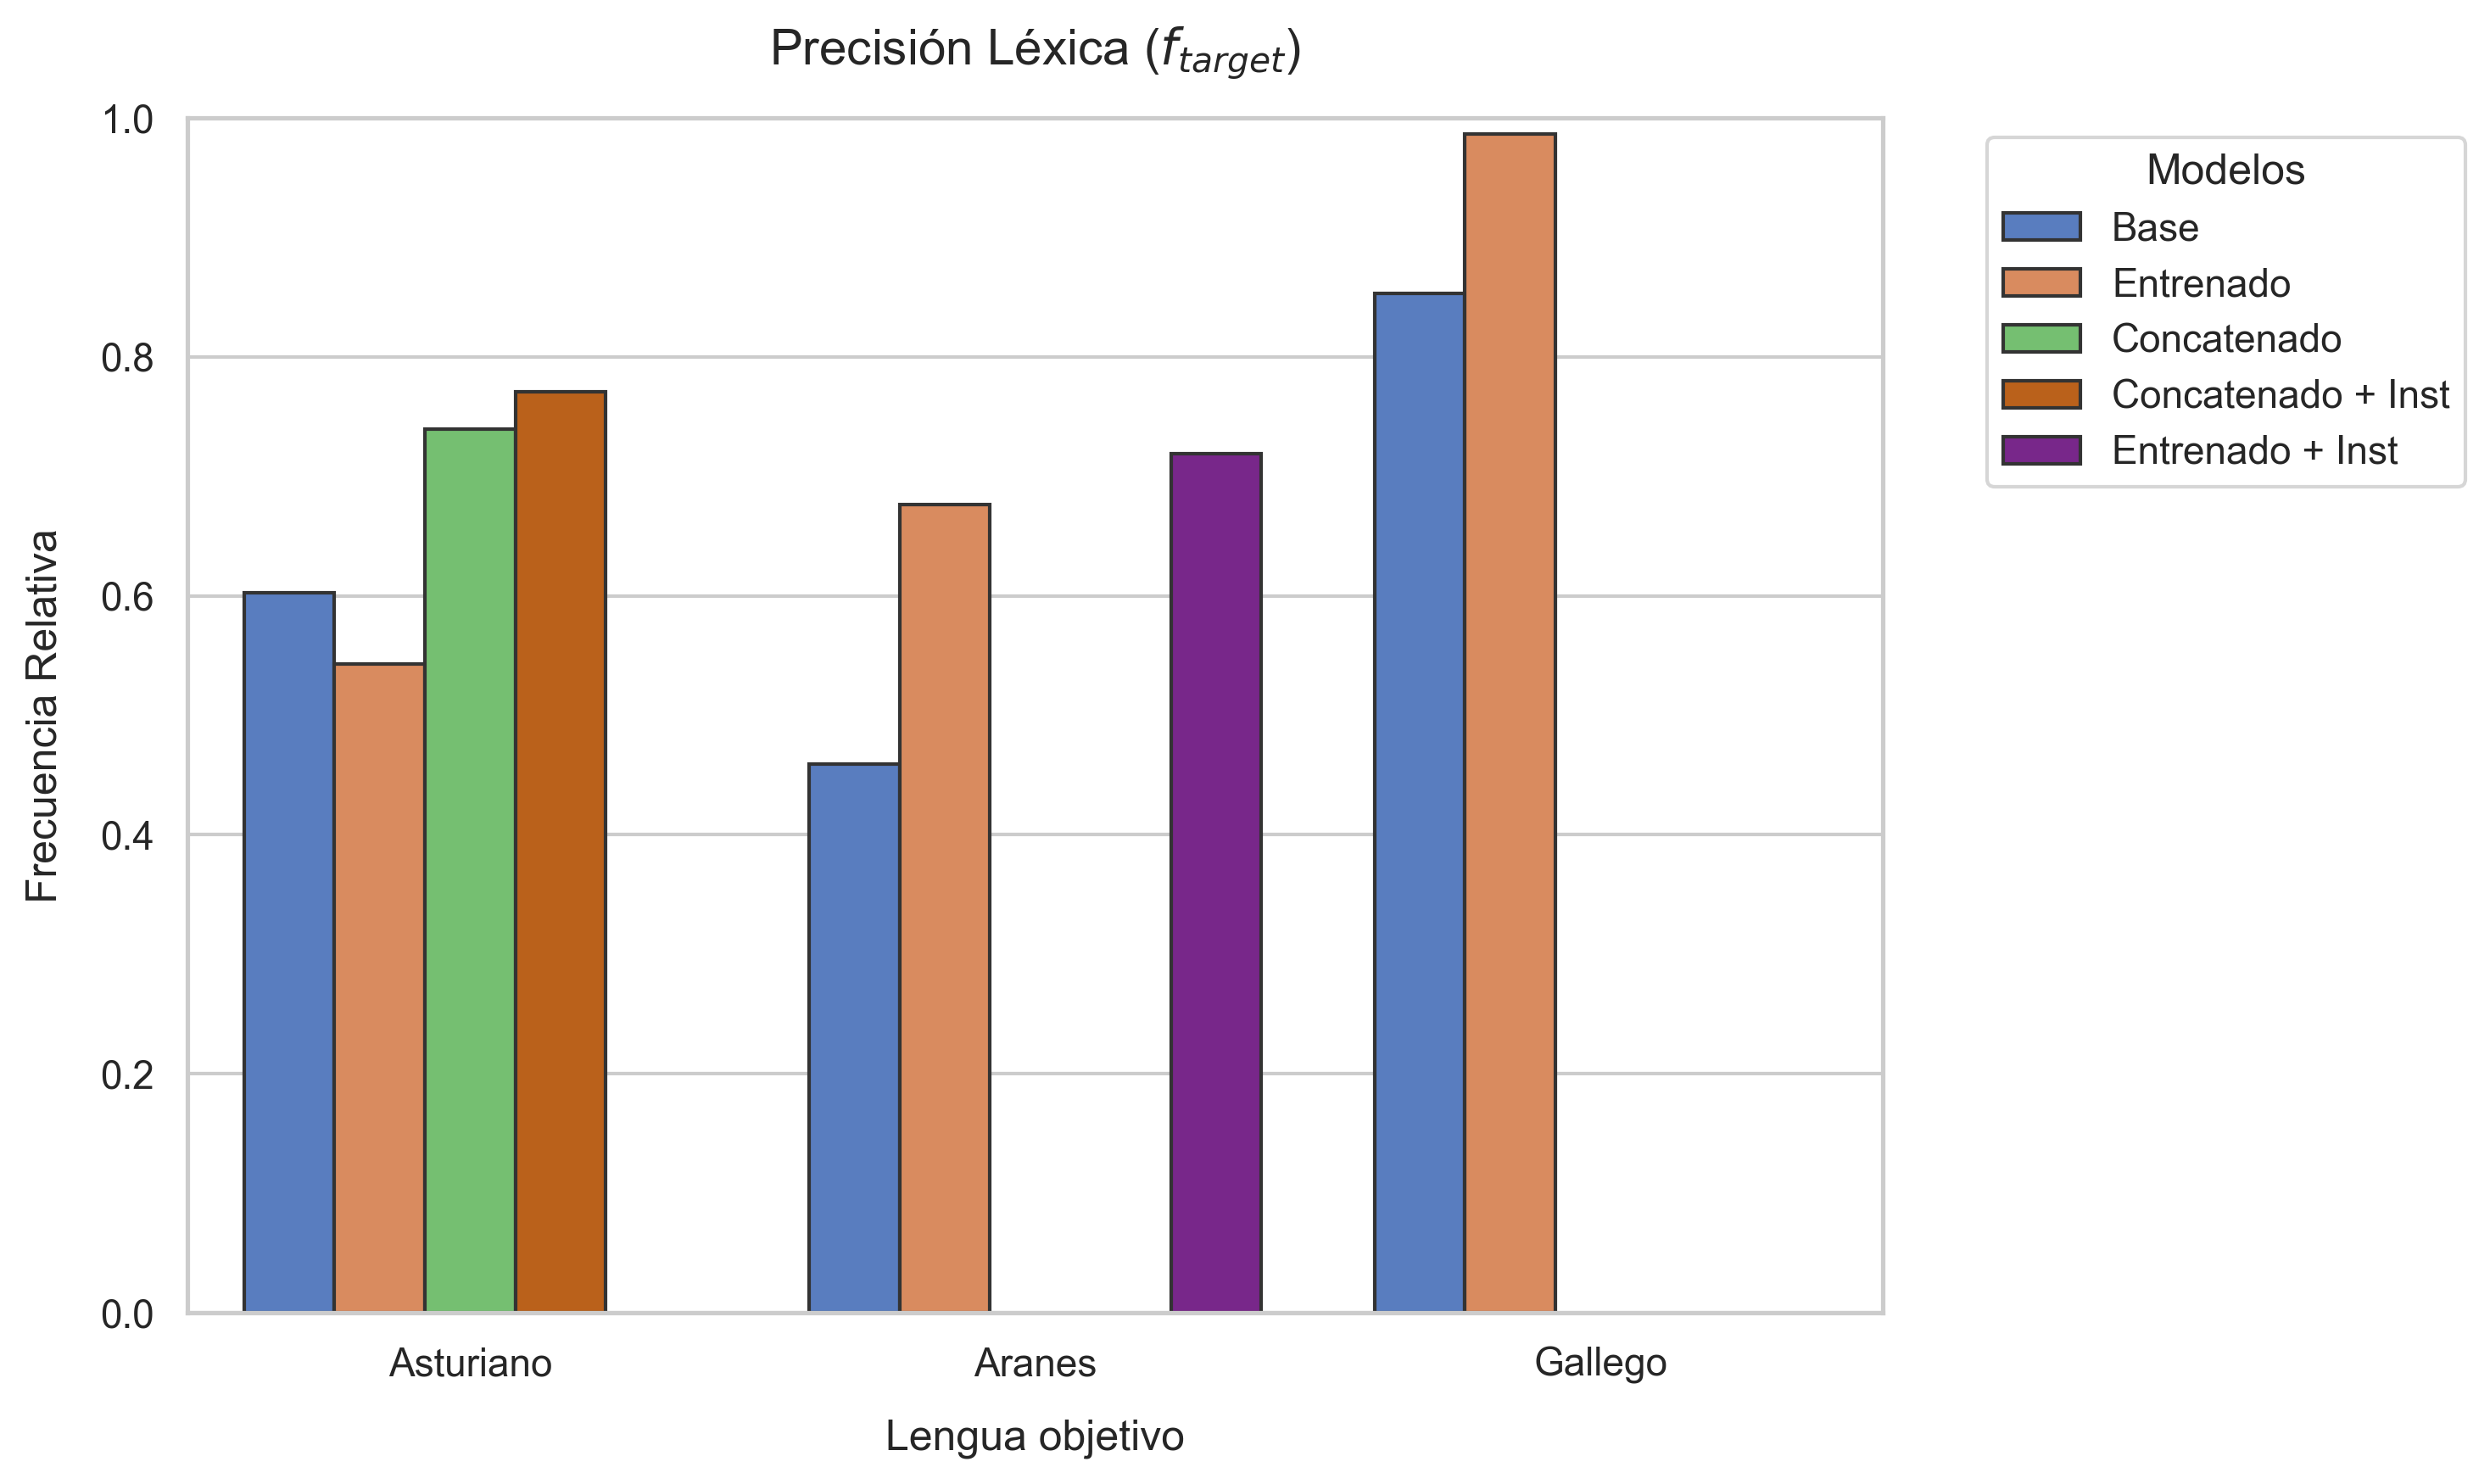
\includegraphics[width=0.8\textwidth]{figures/Calidad_freq_target_qlora.png}    
    \caption{\label{fig:resultados-qlora-freq-target}Freq target de los modelos entrenados por lengua. De creación propia.}
\end{figure}

\textit{En la Figura \ref{fig:resultados-qlora-freq-target} se observa que, en el caso del aranés y del gallego, no se entrenó la versión concatenada debido a la pérdida de coherencia detectada previamente en asturiano. Por tanto, la ausencia de barras en esas lenguas no indica un rendimiento de 0, sino simplemente que esa combinación no fue entrenada.}

En la Figura \ref{fig:resultados-qlora-freq-target} se observa que, en general, todos los modelos entrenados mejoran a sus modelos base en el porcentaje de palabras pertenecientes al diccionario de la lengua objetivo. Destaca especialmente el modelo entrenado en gallego, que pone de manifiesto la importancia de la calidad de los datos: alcanza un 98\% de palabras presentes en el diccionario, una cifra coherente con lo esperable para un modelo que domina la lengua, considerando además posibles ausencias en el diccionario, nombres propios y abreviaturas.
Por otro lado, el modelo entrenado del asturiano es el único que ha bajado de calidad frente a los modelos base.

\begin{figure}[H]
    \centering
    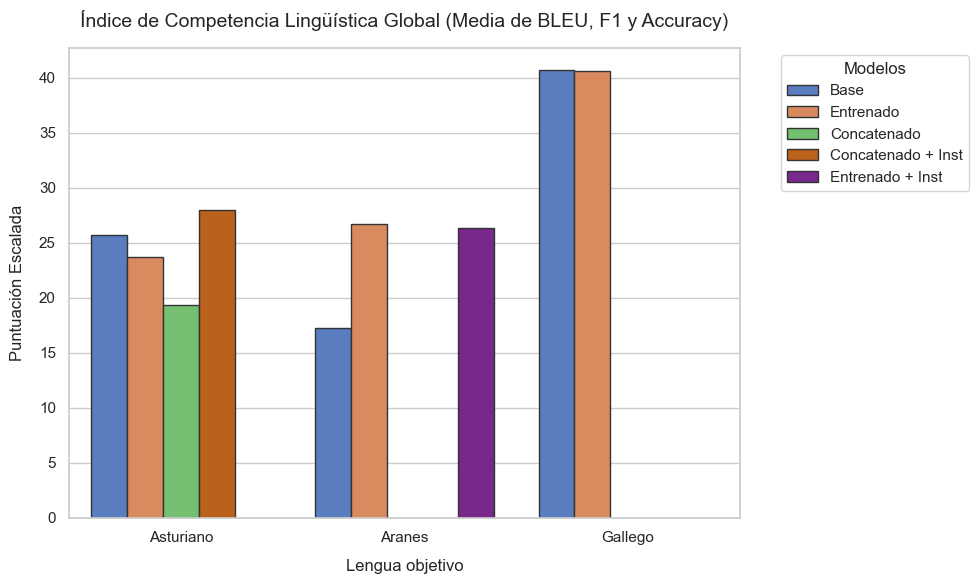
\includegraphics[width=0.8\textwidth]{figures/IndiceMetricas_qlora.png}    
    \caption{\label{fig:resultados-qlora-indice-metricas}Índice global de los resultados de los modelos entrenados por lengua. De creación propia.}
\end{figure}

En la gráfica de media de métricas de evaluación, en la Figura \ref{fig:resultados-qlora-indice-metricas} (calculada como se explicó en \nameref{indice-agrupacion-metricas}) se muestra una mejora de los modelos entrenados, aunque mucho menor, principalmente debido a esa perdida de coherencia. Curiosamente, el modelo que peor funcionaba en el asturiano en freq target, obtiene un mejor resultado que el modelo concatenado en esta métrica, debido a esta perdida de coherencia al concatenar las muestras.

En el gallego, el modelo entrenado mantiene la calidad en este índice, mejorando el número de palabras bien escritas, siendo el mejor resultado del trabajo.

Por último, en el caso del \textit{Aranés}, los resultados muestran mejoras apreciables en ambas métricas, aunque los ejemplos cualitativos revelan que el modelo aún no alcanza un nivel de calidad elevado. Esto sugiere que el modelo base parte de un desempeño especialmente bajo en Aranés, a pesar de la cercanía lingüística con el catalán, y que el entrenamiento consigue una mejora significativa y consistente. Es, de hecho, el caso más llamativo del estudio, es la lengua en la que el modelo más progresa y lo hace de manera más uniforme en ambas gráficas, aunque todavía quede margen para alcanzar una calidad plenamente satisfactoria.
